\documentclass{article}
\usepackage{graphicx}
\usepackage{amsmath}
\usepackage{amssymb}
\usepackage{array}
\usepackage{subfigure}
\parskip 7.2pt
\title{Estimating Markov Random Field Parameters for the model prior}
\author{Alex Kass}
\date{3/20/2011}

\begin{document}
\section{Markov Random Fields}
%
%make .pdf of image
%run to convergence
%describe MRF
%document MRF that we've defined (equations for every function)
%matrix S
%dimensions 245 x length of score
%equations for all features
%p(S) = (...)
%figure with sample input score (with labels corresponding to notation)
%figure (one typical sample from randomly generated score)

A Markov Random Field, or undirected graphical model, provides a representation of non-directional influences among nodes within a network.  Two critical properties of an MRF are conditional independence and factorization, illustrated by the following respective equations:

\begin{eqnarray*}
\Pr(\mathbf{X}) = \prod_i{\Pr(x_i \mid x_{neighbors(i)})}\\
\Pr(\mathbf{X}) = \prod_i{\Pr(x_i, x_{neighbors(i)})}
\end{eqnarray*}

The joint probability of an MRF can be seen as the product of its clique potential energy functions, where a $clique$ is a fully connected subset of nodes, and its potential function $\psi_\theta(x_\theta)$ is 
\begin{eqnarray*}
\psi_\theta(\mathbf{x}_\theta) = \exp\{-E_\theta(\mathbf{x}_\theta)\}
\end{eqnarray*}

Here, $E_\theta$ represents the energy function of a specific clique based on a single parameter $\theta$, and will vary with our MRF parameter constructions as defined in the subsequent section.  We employ the exponentials as a computational convenience, given that our potential functions always represent positive values.  This allows us to calculate the total energy by adding the energies for each of the cliques.  Incorporating $Z(\Theta) = \sum_{\mathbf{x}}\prod_{cliques_\Theta}{\psi_\Theta(\mathbf{x}_\Theta)}$ as the $partition function$, or normalizing constant, we have the joint probability over all nodes $\mathbf{X}$ and cliques $\Theta$ as:
\begin{eqnarray*}
\Pr(\mathbf{X}) = \frac{1}{Z}\prod_{cliques_\Theta}{\psi_\Theta(\mathbf{x}_\Theta)}
\end{eqnarray*}

Thus, to construct our particular MRF, we must define the various potential functions through constructing representations of their respective parameter energy functions.

\section{Defining our MRF parameters and associated elements}

When deciding upon the nature of the parameters of our Markov Random Field, we want to choose both general and specific musical representations.  On the more general side, we've designed one parameter that measures whether a note stays the same or changes (denoted within the model as $\beta$).  In comparison, we designate another parameter ($\lambda$) arbiter of the likelihood of a specific note movement and aggregate all possible note movements within an instrument's four octave range.  Another parameter involves measuring how close a specific voiced note is to the middle of an instrument's range (notated as $\alpha$, utilizing the weighted matrix {\bf M}).  A final set of parameters ($\gamma$) measures the tendencies of certain harmonies to appear within a score - for example, there should be different weights on consonant intervals such as major thirds versus dissonant intervals such as a half-step or a tri-tone (6 half-steps).  On this, we collapse the four-octave range into a single octave (modulo 12 to create a single, 12-note range), so as to emphasize the import of the relative fundamental scale frequencies within an interval's spectrum, rather than to distinguish between three half steps and a minor third three octaves apart.

$S$: A prototype musical Score, in binary matrix form, with $V$ rows and $B$ columns.  When a note is being played, or "on", it is seen as a 1.  If "off", it is 0.

$V$: The range of notes that a quintet can play, concatenating four octaves (=48 notes) and one rest for each instrument part $i$.  Within $S$, $V$ = 245.  $\{1 \le v \le V\}$

$B$: The number of time beats that the score lasts.  This varies from score to score, and is indexed as one beat $b$ per 16th note at common $(4/4)$ musical time.  $\{1 \le b \le B\}$

$\alpha$: A parameter measuring how close a specific voiced note is to the middle of an instrument's range, using the $245x1$ vector {\bf M}, where

$M_v$ = $\{(49\mod{v}) - (V/10)\} / \{(V-10)/10\}$, unless $(49\mod{v}) = 0$, in which case $M_v = 0$.  In calculations, this column vector is concatenated with itself to form a $V$ by $B$ matrix.

$\beta$: A parameter measuring whether a note stays the same or changes.

$\gamma$: A 12x1 vector parameter measuring harmonic intervals within a single octave at any given time point.

$\lambda$: A 95x1 vector parameter measuring note movement intervals between adjancent time points.

{\bf H}: An ordered set of 12 harmonic interval elements that we will interpret as a vector.  {\bf H}: $\{U, m2, M2, m3, M3, P4, TT, P5, m6, M6, m7, M7\}$

{\bf J}: An ordered set of 95 note movement interval elements that we will interpret as a vector.  {\bf J}: $\{-47, -46, \cdots, -1, 0, 1, \cdots, 46, 47\}$


\section{Prototype MIDI Score matrices as parameter training}

We found multiple MIDI quintet scores of different genres to incorporate into a cell array of prototypes with which to initialize our Markov Random Field prior learning process.  To provide a diverse learning environment, these range from classical brass quintets to five-part arrangements of popular tv theme songs.  An example score (an extract from Handel's "Water Music") is seen in Figure 1.

\begin{figure}
\centering
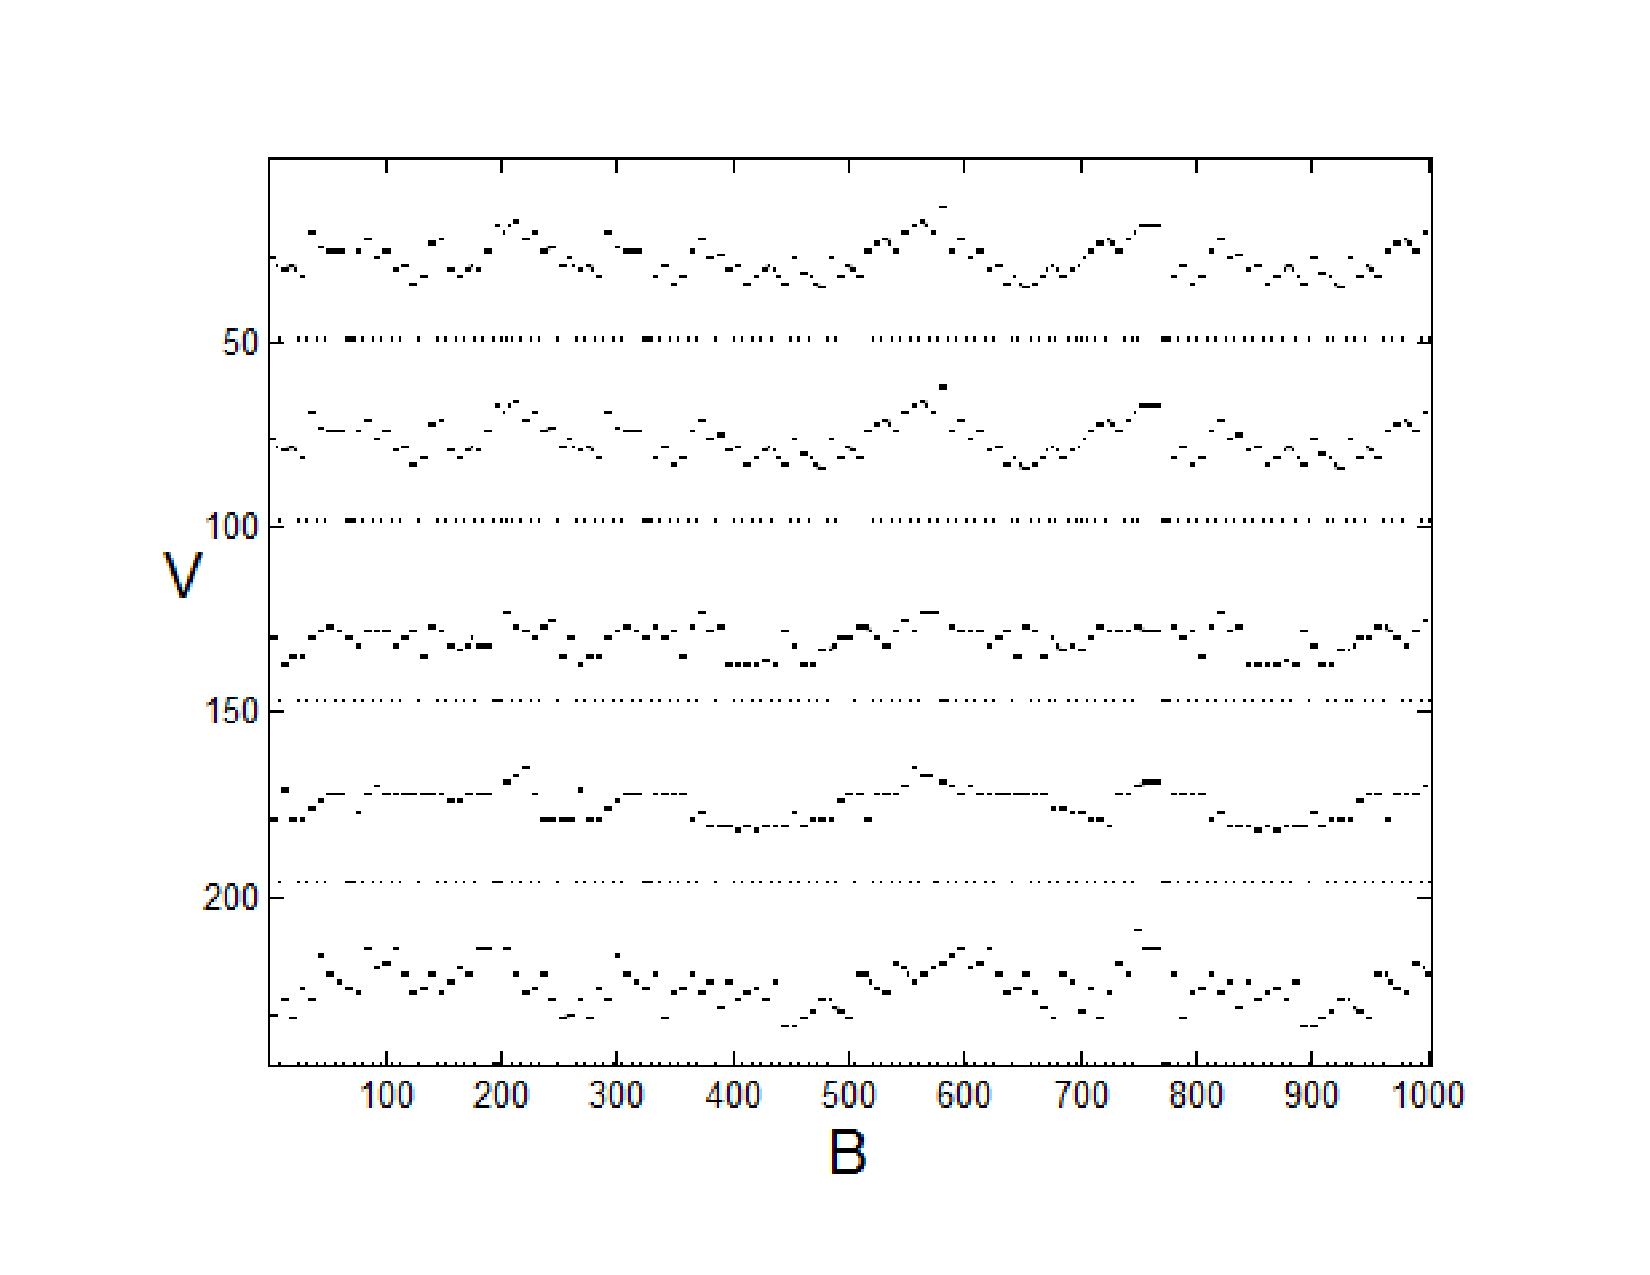
\includegraphics[width=.9\textwidth]{figures/handel(extract).pdf}
\caption{An extract of Handel's "Water Music" in $S$ format, with $V$ = individual pitches for concatenated parts, $B$ = \# of time instances throughout score.  Note the rests occuring every 49th pitch.}
\label{fig-1}
\end{figure}

\section{Learning the MRF parameters for the model prior}

To calculate the joint probability of the score $S$, we multiply together all clique potentials (to follow below) while normalizing by a partition function $Z\left(\Theta\right)$, where $\Theta$ is our joint parameter space:

\[\psi_\alpha = \exp\{-\alpha\sum_{v=1}^V\sum_{b=1}^B{S_{vb}M_{vb}}\}\]
\[\psi_\beta = \exp\{-\beta\sum_{v=1}^V\sum_{b=1}^B{(S_{vb}-S_{v,b-1})^2}\}\]
\[\psi_\gamma = \exp\{-\gamma^\mathrm{T}{\bf H}\}\]
\[\psi_{\bf \lambda} = \exp\{-\lambda^\mathrm{T}{\bf J}\}\]

\[{\bf H} = \sum_{b=1}^B\sum_{i=1}^4\sum_{j=i+1}^5\left(\left|\zeta_{b,i}-\zeta_{b,j}\right|\bmod{12}\in\{U,m2,M2,\cdots,m7,M7\}\right)\]

\[{\bf J} = \sum_{b=2}^B\sum_{i=1}^5\left(\left(\zeta_{b,i}-\zeta_{b-1,i}\right)\in\{-47,-46,\cdots,-1,0,1,\cdots,46,47\}\right)\]

$\zeta_{b,i}$ represents the linear index of the note that is "on" at time $b$ in instrument part $i$.

Thus, the joint is:

\[\Pr\left(S_k|\Theta\right) = \frac{1}{Z\left(\Theta\right)}\exp\{-\alpha\sum_{v=1}^V\sum_{b=1}^B{S_{vb}M_{vb}}- \beta\sum_{v=1}^V\sum_{b=1}^B{(S_{vb}-S_{v,b-1})^2} - \gamma^\mathrm{T}{\bf H} - \lambda^\mathrm{T}{\bf J}\}\]

By taking the $\log$ of both sides of the equation, we can ease computation by simply adding the individual parameter components together within the exponential term on the right side.  We calculate the derivatives of the log of the joint probability for Score $k$ with respect to each of the parameters, then add these together to use as a metric in subsequent Metropolis-Hastings sampling:

%\[\frac{\partial}{\partial\alpha}\log{\Pr\left(S_k|\alpha\right)} = -\frac{1}{Z\left(\Theta_\alpha\right)}\times\left(-\sum_v\sum_b{S_{vb}M_{vb}}\right)\]

\[\frac{\partial}{\partial\alpha}\log{\Pr\left(S_k|\Theta\right)} = \frac{1}{Z\left(\Theta_\alpha\right)}\sum_v\sum_b{S_{vb}M_{vb}}\]

\[\frac{\partial}{\partial\beta}\log{\Pr\left(S_k|\Theta\right)} = \frac{1}{Z\left(\Theta_\beta\right)}\sum_v\sum_b{(S_{vb}-S_{v,b-1})^2}\]

\[\frac{\partial}{\partial\gamma}\log{\Pr\left(S_k|\Theta\right)} = \frac{1}{Z\left(\Theta_\gamma\right)}{\bf H}\]

\[\frac{\partial}{\partial\lambda}\log{\Pr\left(S_k|\Theta\right)} = \frac{1}{Z\left(\Theta_\lambda\right)}{\bf J}\]


%\begin{eqnarray*}
%\lefteqn{\frac{\partial}{\partial\Theta}\log{\Pr\left(S_k|\Theta\right)}}  \\
%&=& \log{\frac{1}{Z\left(\Theta\right)}\exp\{-\alpha\sum_v\sum_b{S_{vb}M_{vb}}- \beta\sum_v\sum_b{(S_{vb}-S_{v,b-1})^2} - \gamma\sum_{b}{H_b} - \lambda^TJ\}}
%\end{eqnarray*}

% write gradient with respect to lambda

%Each 12x1 vector $H^b$ is an aggregate total of harmonic intervals (normalized to fall within a single octave and indexed by $int$) at a specific beat $b$.  It determines all possible pairwise interval combinations from the five notes (${5\choose2}$=10) that are on at a given time step.  $\zeta_i^b$ represents the linear index of the note that is "on" at time $b$ in instrument part $i$:
%
%\[H_{int}^b = \sum_{i=1}^4\sum_{j=i+1}^5\mathbb{1}\left(\left|\zeta_i^b-\zeta_j^b\right|\bmod{12} = int\right)\]
%
%As seen above, the $\lambda$ parameter (this being a 95x1 vector) is multiplied by $J$, which itself is a vector of the sums of each of the 95 interval jumps (here indexed as $int$), tabulated within each of the five instruments ($i$) throughout the duration of the score.  Thus, $\zeta_{b,i}$ holds similar information as the preceding equation:
%
%\[J_{int} = \sum_{b=2}^{B}\sum_{i=1}^5\mathbb{1}\left(\left|\zeta_{b,i}-\zeta_{b-1,i}\right| = int\right)\]


\section{Estimating parameters through MCMC and Contrastive Divergence}
We employ a Metropolis-Hastings sampler to draw from the array of prototype scores, updating each of the parameters accordingly.  Further, using Contrastive Divergence, we move the parameter estimates along towards convergence via gradient ascent, employing the notion that the a single parameter's component of the gradient is proportional to the difference between the expectation of the log of the derivative with respect to that parameter over the original score data and that of the newly sampled score data.  Referencing the combined parameter space $\Theta$, and moving along the gradient so as to minimize the energy function of the MRF, we have the update function:

\[\Theta_{t+1} = \Theta_t + \eta\nabla_{\Theta}\]

where $\eta$ is the set of learning rates for the parameters, determined experimentally, and

\[\nabla_{\Theta} = \langle\frac{\partial\log{f(x;\Theta)}}{\partial\Theta}\rangle_{X^0} - \langle\frac{\partial\log{f(x;\Theta)}}{\partial\Theta}\rangle_{X^s}\]

Contrastive divergence allows us to approximate the gradient for the parameters by iterating only a few times through the MCMC process, which speeds up computation considerably.  In the above equation, $X^s$ represents the $s$th iteration of sampling the data {\bf X}.

Once the parameters have been estimated to the point of convergence, we set them as the prior and proceed to subsequent signal processing.  Figure 2 shows the convergence of the $\beta$ and "M3," or "major 3rd" component of the $\gamma$ harmonic interval vector over 40,000 iterations of sampling.  We measured convergence based on the asymptotic movement of the joint log likelihood and norm of the gradient.

\begin{figure}
\centering
\mbox{
\subfigure{
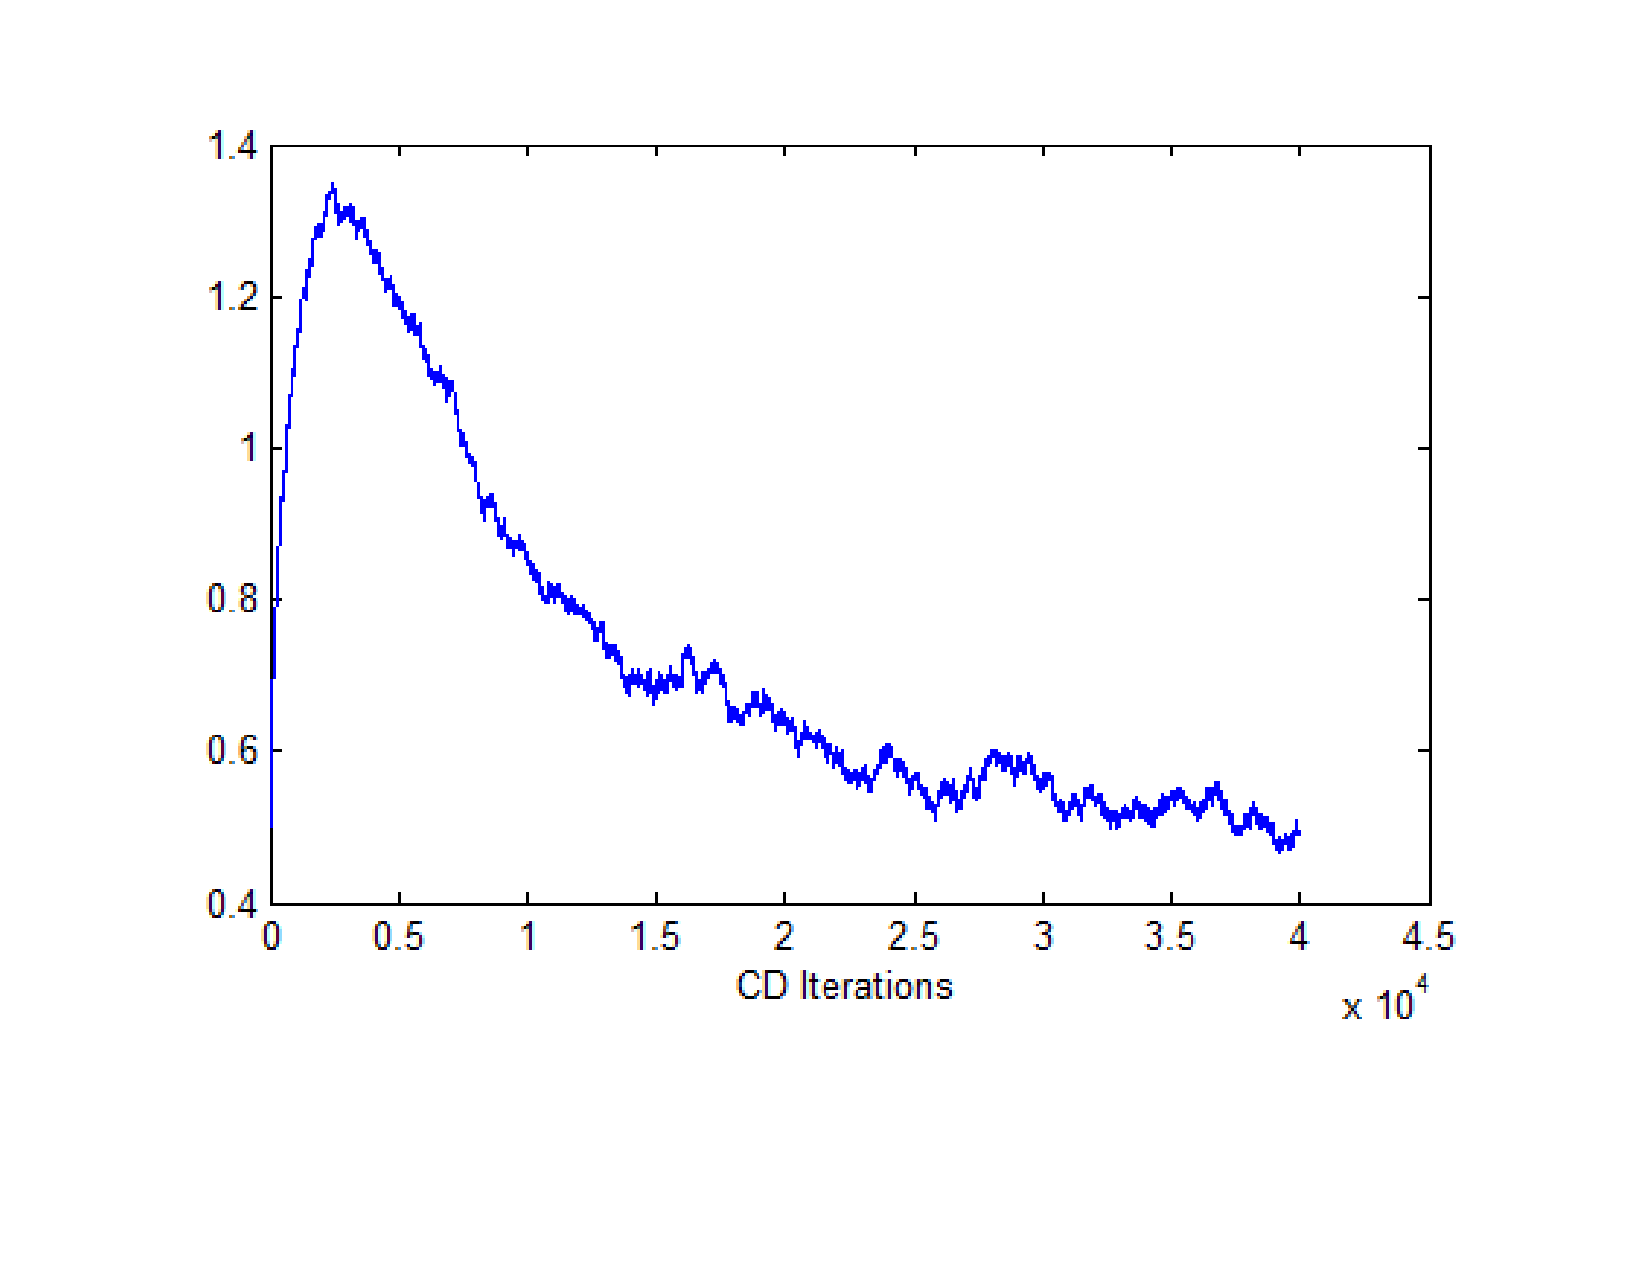
\includegraphics[width=.25\textwidth]{figures/alpha.pdf}
\label{fig-2}
}\quad
\subfigure{
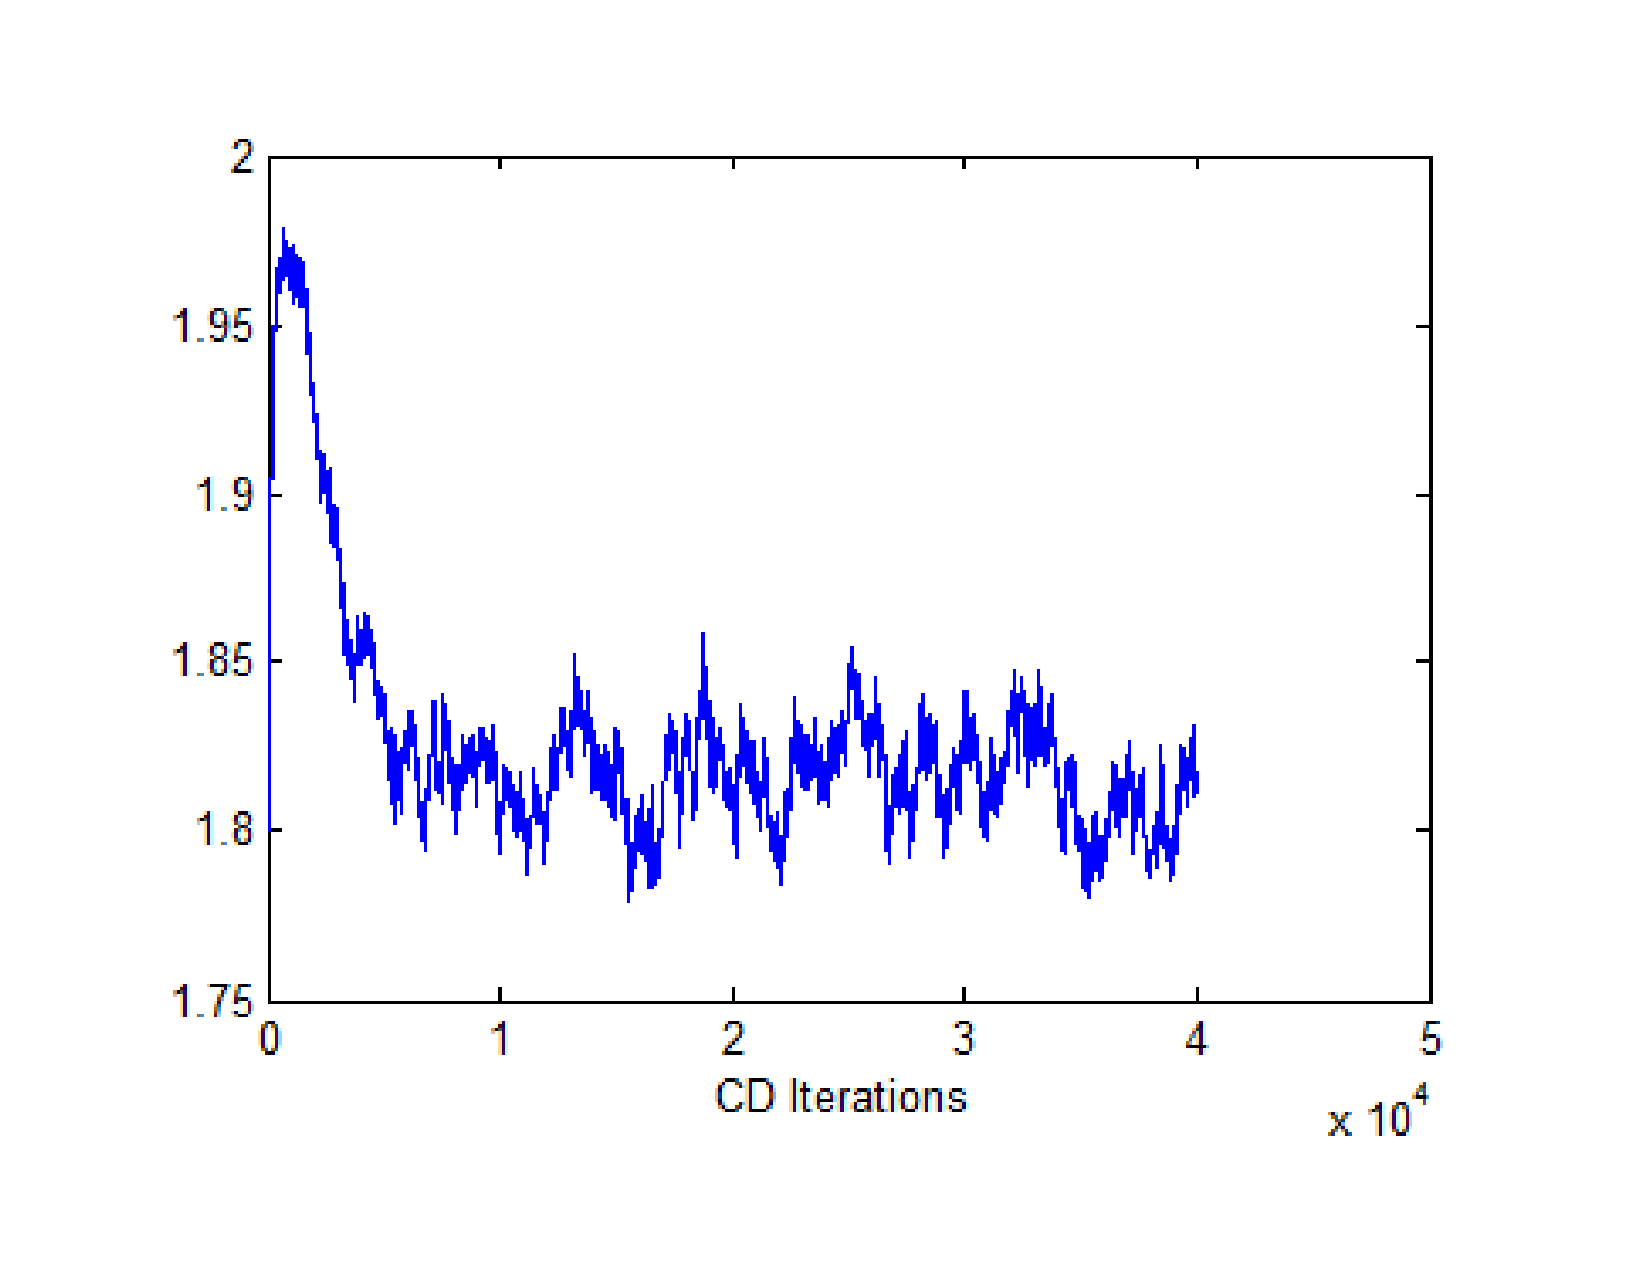
\includegraphics[width=.25\textwidth]{figures/beta.pdf}
\label{fig-3}
}\quad
\subfigure{
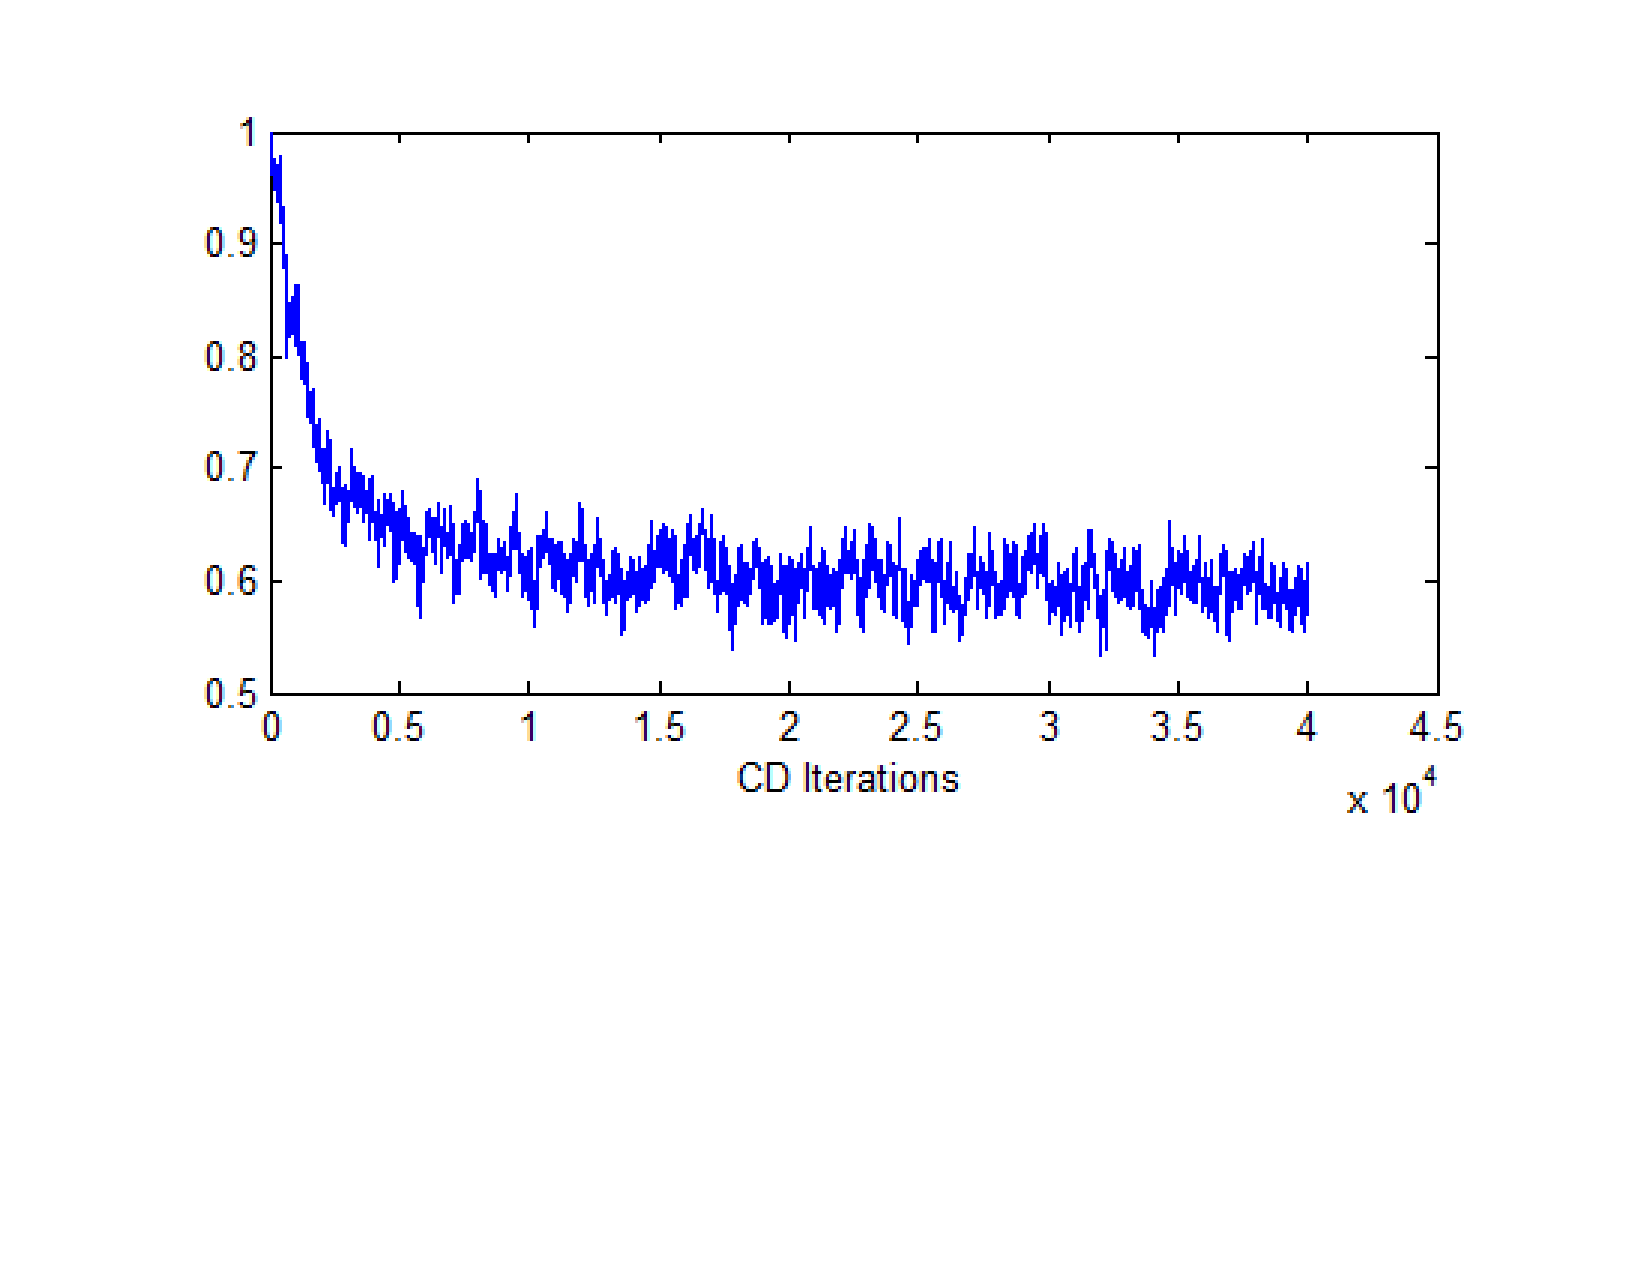
\includegraphics[width=.25\textwidth]{figures/harmony(M3).pdf}
\label{fig-4}
}\quad
\subfigure{
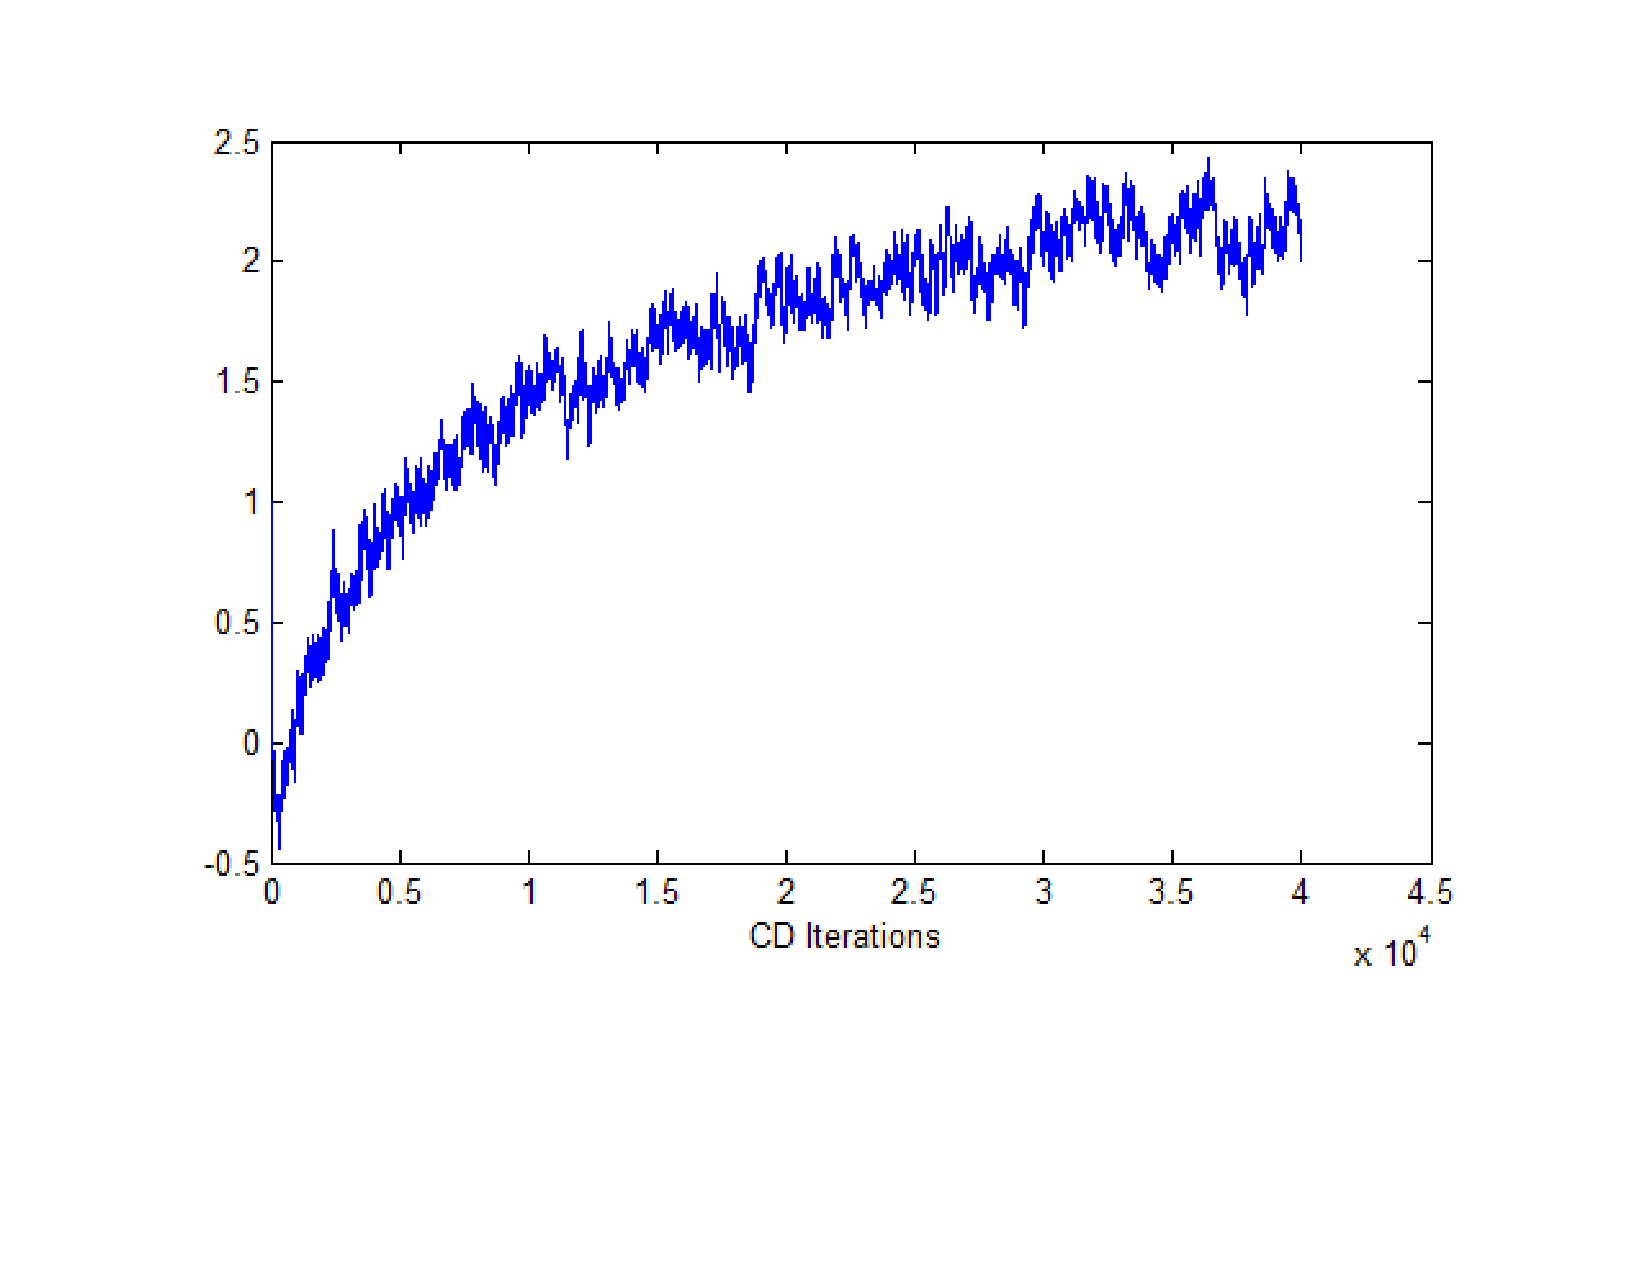
\includegraphics[width=.25\textwidth]{figures/note_movement(downhalfstep).pdf}
\label{fig-5}
}
}
\centering
\caption{Convergence of $\alpha$, $\beta$, $\gamma$ (Major 3rd interval), and $\lambda$ (down 1/2 step) parameters over 40,000 sampler iterations using 3 Contrastive Divergence sweeps per sample.}
\label{fig-all}
\end{figure}

We can demonstrate the effect of our learned parameters by generating a random score and observing the same score after it has been sampled 1000 times using the new parameters, as seen in Figure 3.

\begin{figure}
\centering
\mbox{
\subfigure{
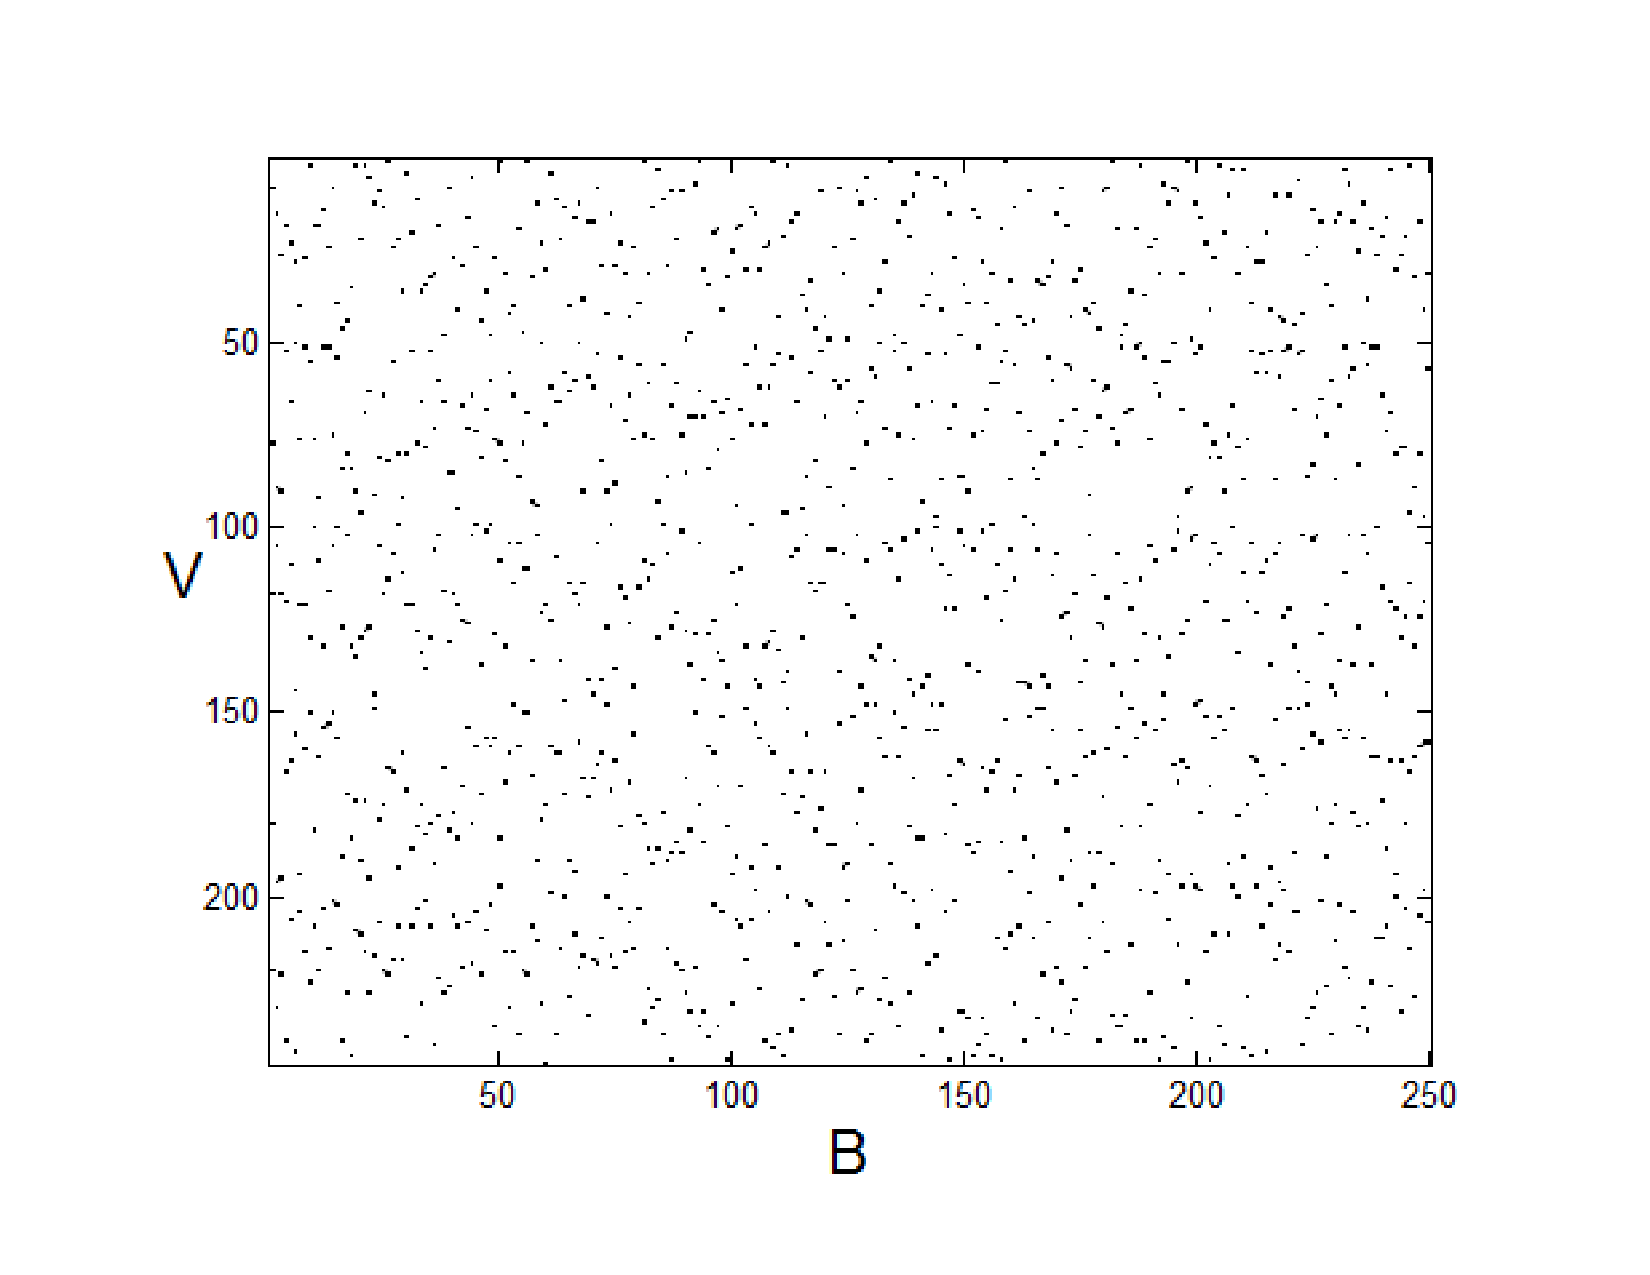
\includegraphics[width=.5\textwidth]{figures/Score(Random).pdf}
\label{fig-6}
}\quad
\subfigure{
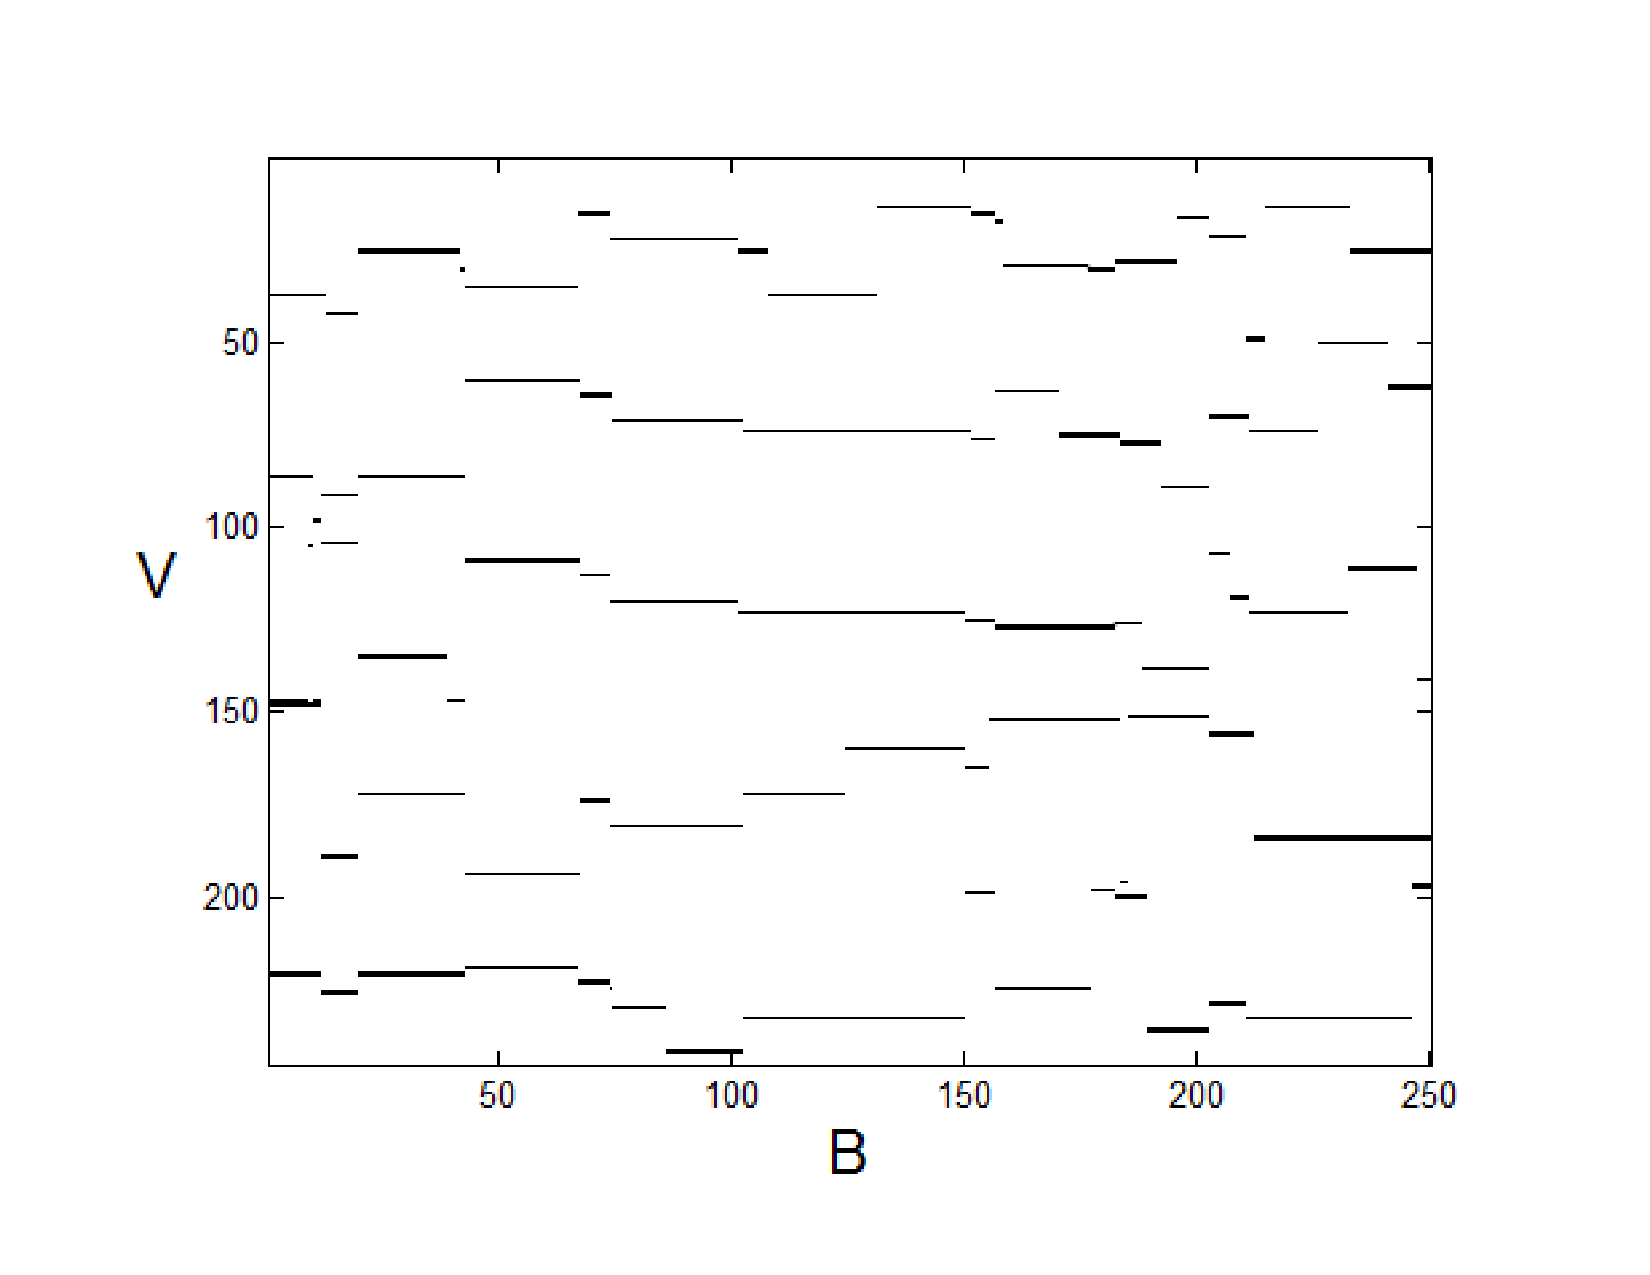
\includegraphics[width=.5\textwidth]{figures/Score(Sampled).pdf}
\label{fig-7}
}
}
\centering
\caption{Comparison of Randomly Generated Score and this same Score after sampling}
\label{fig-all}
\end{figure}

\begin{figure}
\centering
\mbox{
\subfigure{
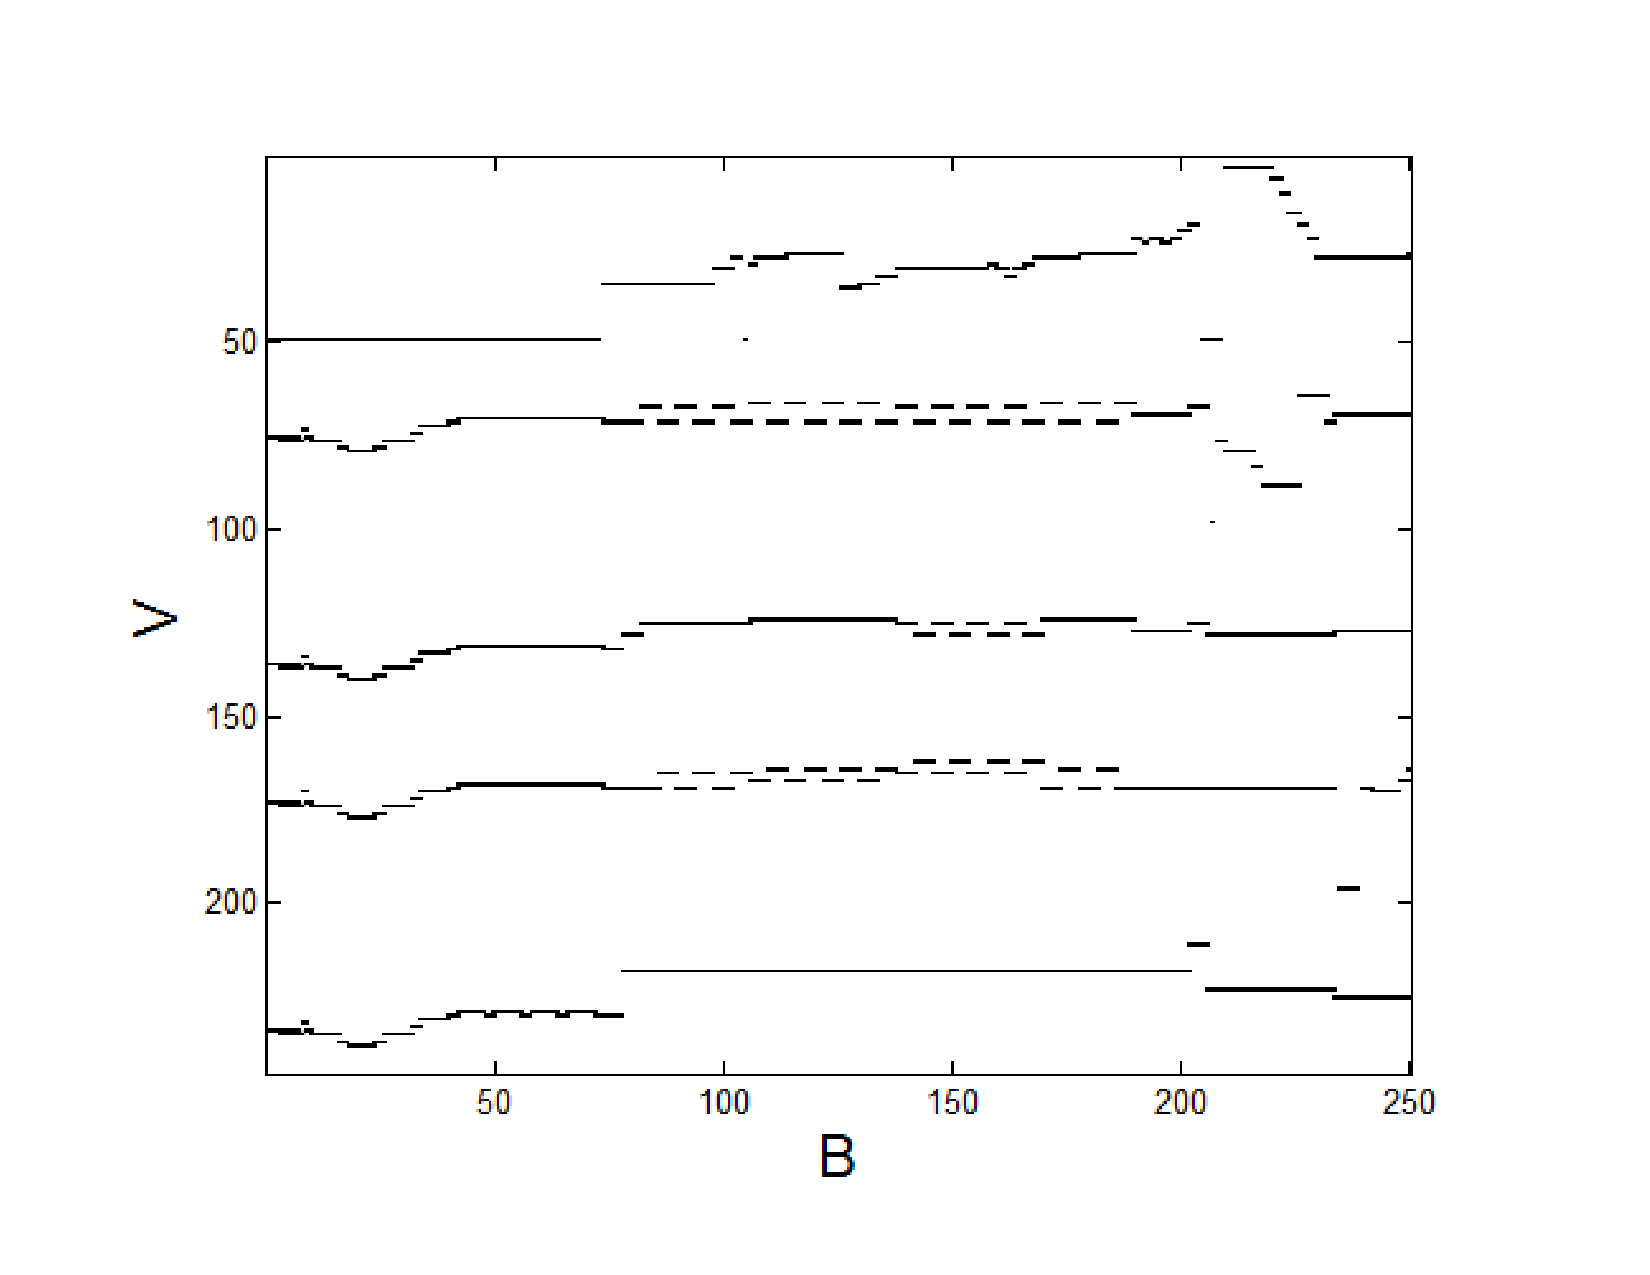
\includegraphics[width=.5\textwidth]{figures/Score(Weber-Original).pdf}
\label{fig-8}
}\quad
\subfigure{
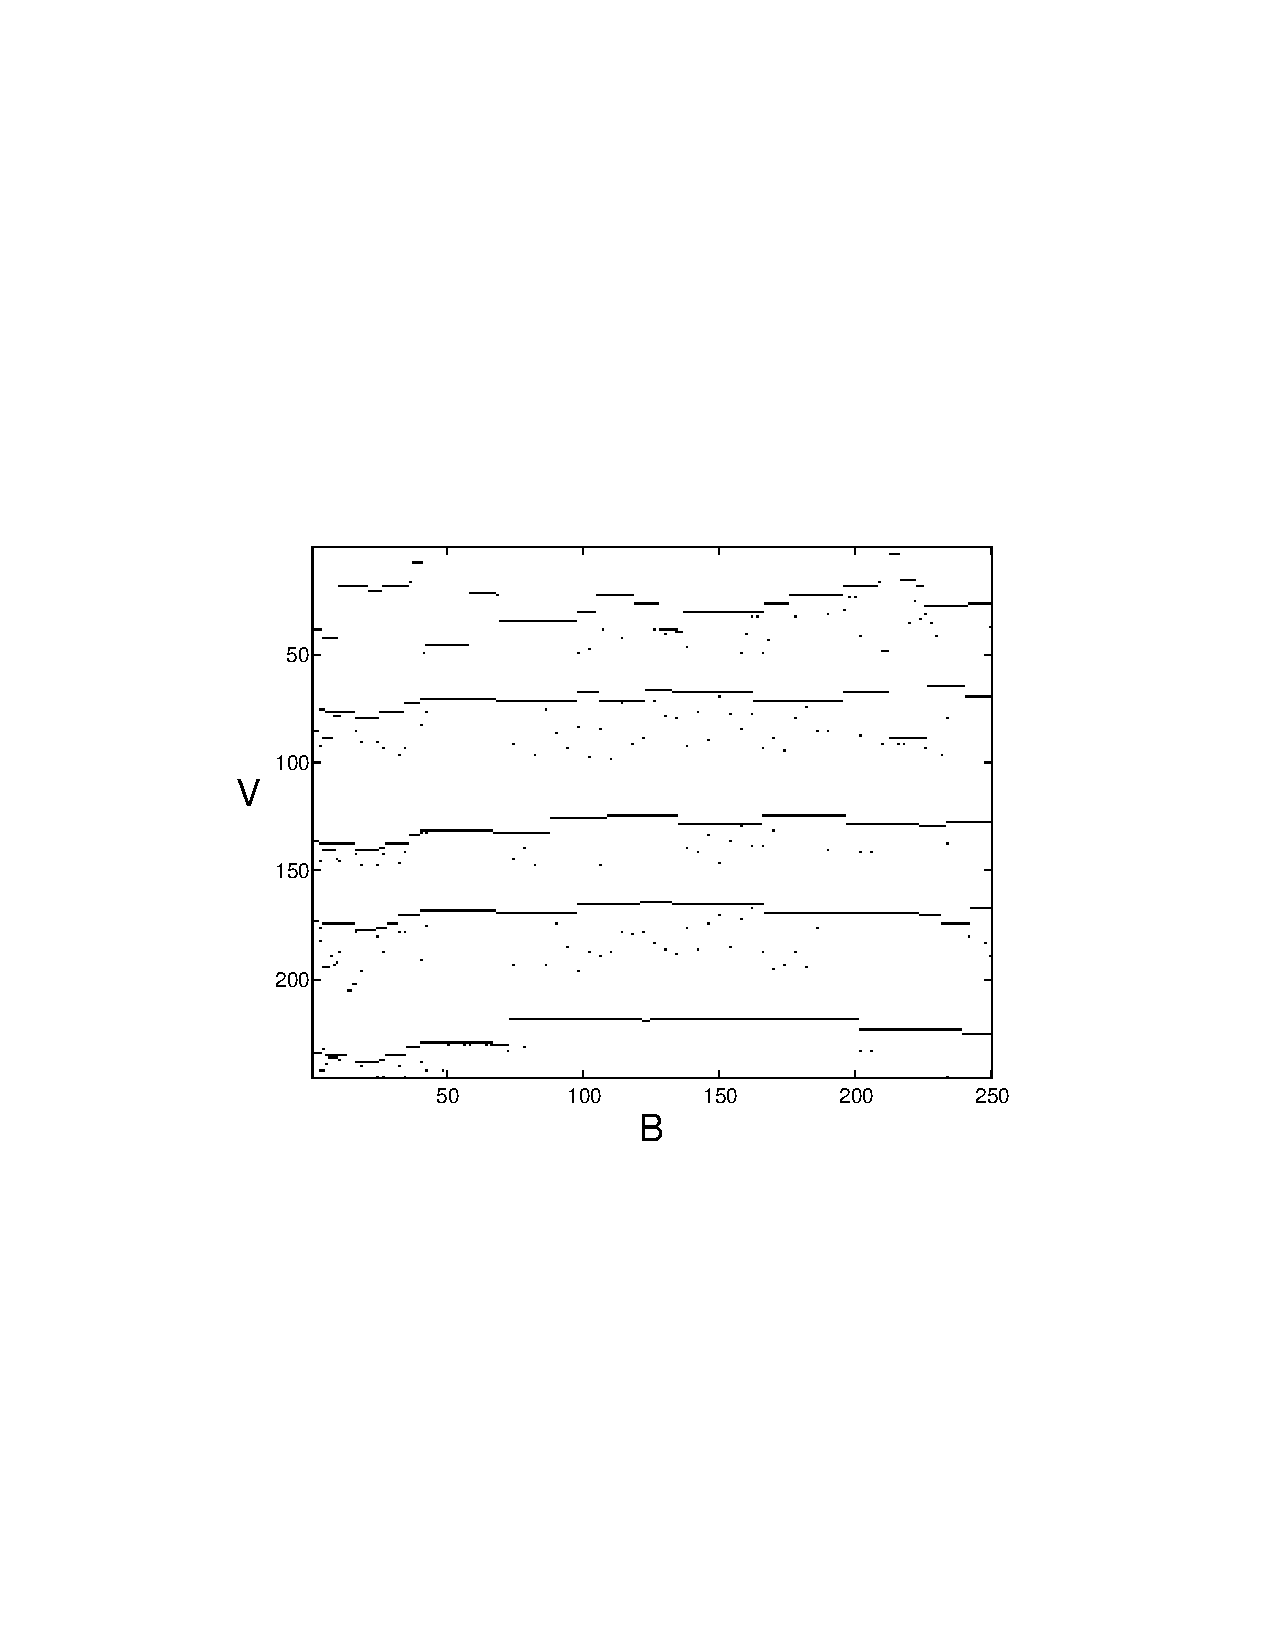
\includegraphics[width=.5\textwidth]{figures/Score(Weber-Sampled).pdf}
\label{fig-9}
}
}
\centering
\caption{Comparison of one actual score and this same score after sampling}
\label{fig-all}
\end{figure}


\section{Conclusions}
Comparing a randomly-generated score and the same score after sampling, it is clear that the learned parameters are affecting the score.  The sampling does well to elongate individual notes and to cluster sequences of these longer notes close to each other within each instrument scale.

When observing an original, prototype score before and after it has been sampled using our learned parameters, we can see that certain properties have been preserved, while others have been deemphasized.  In particular, the long, held notes do not seem to move from their original positions (unless they were initially in the rest position), whereas the shorter notes are somewhat elongated (e.g. a long series of alternating short notes are combined into a single long note or longer series of fewer alternating notes).  Additionally, the sampled model contains noise in the form of 1 beat-length notes at seemingly random harmonic intervals.

One possible addition to the parameter set might include a parameter governing specifically when to populate the rest (i.e. non-playing) rows.  Further, we may design a parameter that combines the characteristics of the harmony and note movement parameters (currently $\gamma$ and $\lambda$, respectively), essentially embodying the "voice-leading" rules of Western composition.

Another avenue of expansion would be to include prototype scores from non-Western genres, or perhaps even to learn a specific set of parameters when given a target score.  For example, if a user wishes to learn a score from a particular genre, we could feed the parameter-learning algorithm a modified set of prototypes to better reflect the musical target.



\end{document}